\section{A brief history of DNA}

In the winter of 1868/9, Swiss physician and biologist, Johannes Friedrich Miescher isolated an unknown substance from the nuclei of cells\cite{dahm2008discovering}. This substance was unlike anything he had observed before; it was resistant to protease, lacked sulphur, and contained a large amount of phosphorous. He recognised that he had isolated a novel substance and as it was from the nucleus, he named it nuclein. In 1881, Albrecht Kossel determined that nuclein was composed of five bases: adenine (A), cytosine (C), guanine (G), thymine (T), and uracil (U). Later in 1889, Richard Altmann discovered that nuclein was acidic (due to the presence of phosphorous) and renamed nuclein to nucleic acid. The basic component of deoxyribonucleic acid (DNA) was deduced by Phoebus Levene in 1909, where he discovered that DNA consisted of an acid, an organic base, and a sugar. Levene also showed that these components were linked together as phosphate-sugar-base to form units, which he termed nucleotides. This sugar-phosphate backbone forms the structural framework of nucleic acids and makes DNA highly stable. In 1928, Frederick Griffith demonstrated that heritable traits could be transferred between dead and live bacteria and that provided the first clue that a ``transforming factor" existed\cite{griffith1928significance}. It wasn't until 1944, when Oswald Avery, Colin MacLeod, and Maclyn McCarty demonstrated that deoxyribonucleo-depolymerase (an enzyme that degrades DNA) destroyed the ``transforming factor", that it was hypothesised DNA was the genetic material\cite{avery1944studies}. This was later confirmed in 1952 by Alfred Hershey and Martha Chase, by demonstrating that when bacteriophages infected bacteria, only their DNA would enter into the cytoplasm of the bacteria, while their protein remained outside\cite{hershey1952independent}.

While Levene proposed that DNA was made up of equal amounts of A, C, G, and T, it was later discovered by Erwin Chargaff that DNA had a one-to-one ratio of pyrimidine (C, T, and U) and purine (A and G) bases\cite{pmid14938364, pmid14945441}; this became known as Chargaff's rules. This observation by Chargaff and an X-ray diffraction image taken by Rosalind Franklin was necessary for the deduction of the three-dimensional (3D) structure of DNA by Francis Crick and James Watson in 1953\cite{WATSON_1953} The 3D structure of DNA demonstrated how adenines paired with thymines and cytosines paired with guanine (Figure ~\ref{fig:dna}); this is known as Watson-Crick base pairing and explained how genetic information could be copied due to the complementary nature of DNA.

\begin{figure}[!ht]
   \centering
   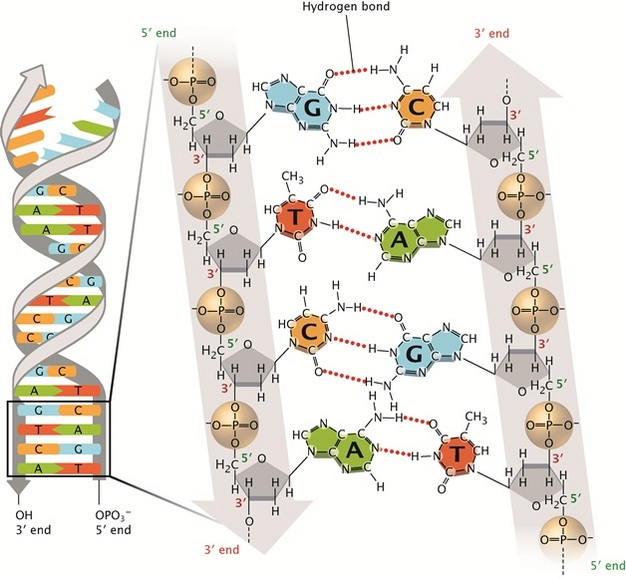
\includegraphics[width=\textwidth,natwidth=626,natheight=579]{dna_scitable.jpg}
   \caption[DNA base pairing]{The structure of DNA is based on the repeated pattern of deoxyriboses and phosphate groups, forming the sugar-phosphate backbone, and the base pairing of the four bases, adenine (A), cytosine (C), guanine (G), and thymine (T). Two hydrogen bonds connect A to T and three hydrogen bonds connect C to G. Image used with permission from Nature Education 2013.}
   \label{fig:dna}
\end{figure}

\section{The Central Dogma of Molecular Biology}

In 1958 Francis Crick wrote a seminal paper on protein synthesis, where he described the importance of proteins in living organisms and first proposed the central dogma of molecular biology\cite{crick1958protein}. Crick described how DNA or ribonucleic acid (RNA) could be used as templates for proteins and further described the possible directions of information flow between DNA, RNA, and protein. However, he noted that once information had been transferred from either DNA or DNA to protein, it is not possible for information to flow back to nucleic acids. In 1970, an enzyme known as reverse transcriptase (RT) was discovered\cite{pmid4316301,pmid4316300}, which allows RNA to be used as a template for producing DNA. In light of this and due to the misunderstanding of the central dogma, Crick restated the central dogma\cite{CRICK1970}:

\epigraph{``The central dogma of molecular biology deals with the detailed residue-by-residue transfer of sequential information. It states that such information cannot be transferred from protein to either protein or nucleic acid."}{--- \textup{Francis Crick 1970}}

\begin{figure}[!ht]
   \centering
   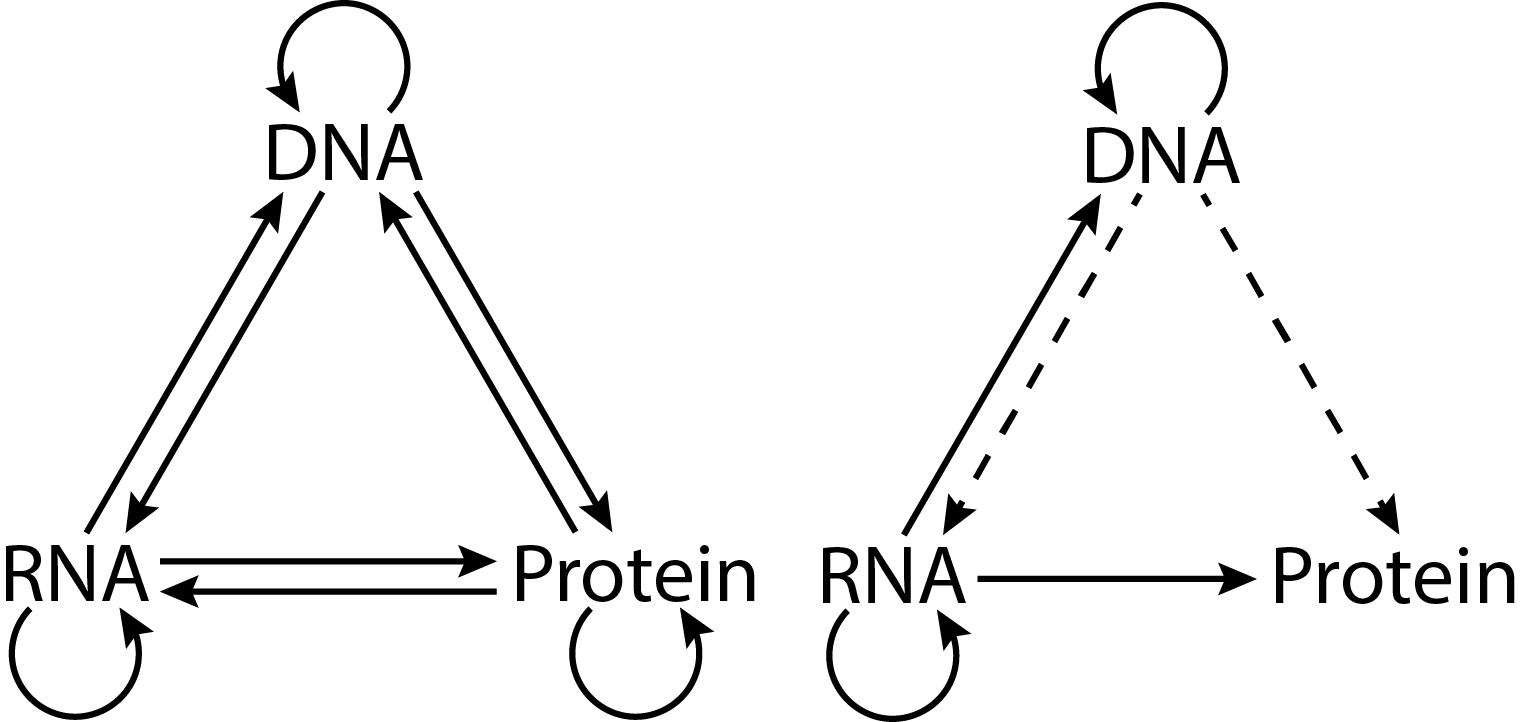
\includegraphics[width=\textwidth,natwidth=1520,natheight=722]{central_dogma.png}
   \caption[The central dogma]{All possible information transfer pathways between DNA, RNA, and protein are shown on the left. Probable (solid arrows) and possible (dotted arrows) information transfer pathways, as originally proposed in 1958 by Francis Crick\cite{crick1958protein}, are shown on the right. Note that once information has been transferred to a protein, it is not possible for this information to be transferred back to nucleic acids, which is known as the central dogma of molecular biology.}
   \label{fig:central_dogma}
\end{figure}

Prior to proposing the central dogma, Crick had predicted the existence of ``adaptors" that would transfer information from RNA to protein in 1955\cite{cricktrna1955}. Crick had proposed that there were twenty adaptors and special enzymes, one for each amino acid; the enzyme would join one particular amino acid to its own special adaptor. This theory was later confirmed by the discovery of transfer RNA (tRNA) in 1958\cite{pmid13538965}. The discovery of messenger RNA (mRNA) in 1961 \cite{BRENNER1961} demonstrated the flow of information from DNA to RNA and subsequently to the ribosomes\cite{pmid14381428} for protein synthesis. In 1962, the code used by DNA to encode the amino acids of proteins was deduced  by the use of artificial RNA and bacteria\cite{pmid14471390}. Matthaei and colleagues demonstrated that an artificially created RNA, composed entirely of uracils, would produce a protein composed entirely of the amino acid phenylalanine. The full code, known as the genetic code, was cracked three years later in 1965\cite{pmid5330357} and defined how information is encoded in DNA. Nirenberg and colleagues deduced that three nucleotides defined a codon, which are translated into one of the 20 standard amino acids.

\section{Transcription}

Transcription is the process by which a particular segment of DNA is processed into RNA by the enzyme RNA polymerase (RNA pol). There are three different types of RNA polymerases in eukaryotic cells: Pol I transcribes DNA that encode most of the ribosomal RNAs (rRNAs); Pol II transcribes DNA that encode mRNAs and other non-coding RNAs; and Pol III transcribes the genes for small regulatory RNA molecules, such as tRNAs. The first step in transcription is initiation, whereby RNA pol binds upstream of the DNA to be transcribed, at a region known as the promoter (Figure ~\ref{fig:transcription}). Promoters can be classified by their distance from the transcription start site (TSS), which are the first nucleotides transcribed by RNA pol. The core promoter for a region to be transcribed, i.e. the transcript, by Pol II is usually found immediately upstream of the TSS and contains specific DNA sequences or elements that are necessary for transcription. The core promoter elements include the TATA box (usually located 25 to 35 bases upstream of the TSS), the TFIIB recognition element [also known as the B recognition element, (BRE)], the initiator element (Inr), the downstream promoter element (DPE), and CpG islands (CGIs) (Figure ~\ref{fig:core_promoter}). The proximal promoter lies $\sim~250$ bp of the TSS and contains primary regulatory elements. Distal promoters do not have a fixed distance from the TSS but are usually further upstream and contain additional regulatory elements.

\begin{figure}[!ht]
   \centering
   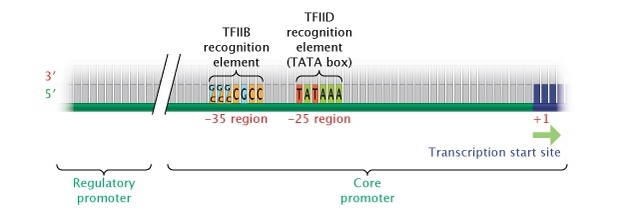
\includegraphics[width=\textwidth,natwidth=626,natheight=216]{core_promoter.jpg}
   \caption[Core promoter elements]{Core promoter elements recognised by Pol II include the TFIIB recognition element and the TATA box, which are located around 35 and 25 bp upstream of the transcription starting site (TSS), respectively. Regulatory elements lie further upstream of the TSS. Image used with permission from Nature Education 2014.}
   \label{fig:core_promoter}
\end{figure}

Once transcription has initiated, RNA pol and its associated proteins unwind the DNA double helix; once unwound, RNA pol reads the template DNA strand and adds nucleotides to the 3' end of a nascent RNA transcript. Transcription is terminated when the RNA polymerase reaches the termination site and the mRNA transcript and RNA pol are released (Figure ~\ref{fig:transcription}). Transcription results in two main classes of RNA transcripts: (1) Protein-coding transcripts, where the RNA known as mRNA can be further translated into a protein molecule and (2) Non-coding transcripts, where the RNA molecule is the functional product.

\begin{figure}[!ht]
   \centering
   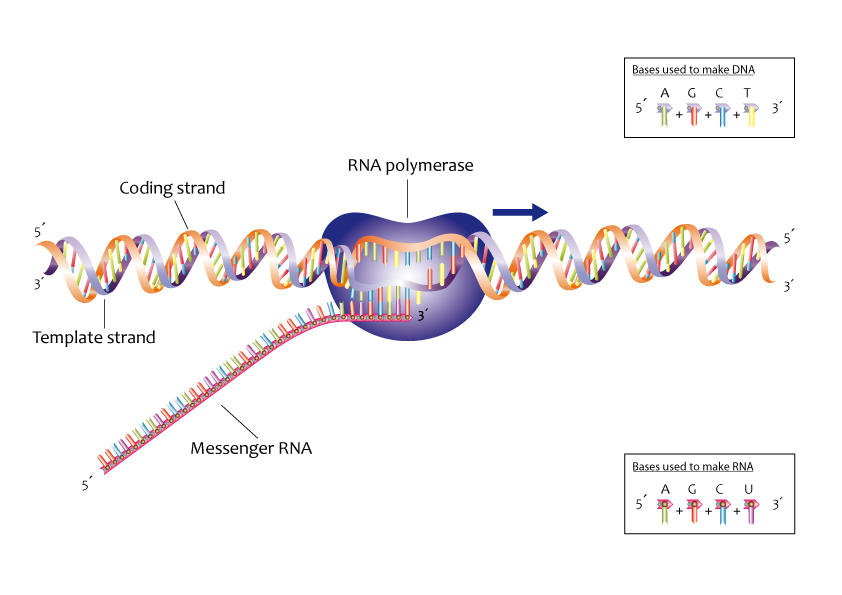
\includegraphics[width=\textwidth,natwidth=842,natheight=595,totalheight=0.70\textheight,keepaspectratio]{transcription.jpg}
   \caption[DNA transcription]{The process of transcription can be broadly grouped into three stages: a) initiation, b) elongation, and c) termination. Initiation involves the binding of RNA polymerase (shown as a large green blob) to the promoter and the DNA double helix starts to separate. RNA polymerase starts reading the sequence on the template strand in the 5' to 3' direction (green arrow). The elongation step involves the movement of RNA polymerase along the DNA strand producing a growing RNA transcript chain, which continually closes and opens the DNA strand. The nucleotides are shown as pink T-shaped molecules and the red arrow indicates that they are added at the 3' end of the nascent transcript. Once the RNA polymerase reaches the termination site, the RNA transcript and RNA polymerase are separated from the DNA. Image used with permission from Nature Education 2013.}
   \label{fig:transcription}
\end{figure}

\subsection{Transcriptional regulation}

The regulation of transcription ensures that transcripts are expressed in the correct spatial and temporal manner; this is necessary for maintaining cellular identity and for responding appropriately to environmental cues. Transcriptional regulation is achieved mainly through the interaction of proteins called transcription factors (TFs) and through the structural packaging of DNA. TFs are regulatory proteins that can activate or enhance the transcription of DNA by binding to specific DNA sequences and recruiting RNA polymerase\cite{pmid11092823}. TFs contain DNA-binding domains (DBDs) that enable it to bind specifically to DNA regions; these sites are known as transcription factor binding site (TFBS). One particular group of regulatory DNA sequence that TFs bind to are enhancer sequences, which when bound to leads to an enhancement in the rate of transcription. Enhancer sequences can be located thousands of nucleotides away from the promoter they interact with, as they are brought into proximity to the promoter by the physical looping of DNA. In addition, enhancers may be positioned in both forward and reverse orientations, and located either upstream or downstream from its associated promoter and still affect transcription.

The structural compaction of DNA into chromosomes limits the accessibility of DNA to TFs and RNA pol. This compaction is achieved mainly via histones, which are a family of small and positively charged proteins that fold negatively charged DNA in the form of electrostatic interactions; this folding helps condense DNA and the resulting DNA-histone complex is called chromatin. Chromatin possesses a fundamental repeating structure\cite{holde01111974}, known as the nucleosome, which is the structural and functional unit of chromatin. Nucleosomes are structured with two of each of the following histones: H2A, H2B, H3, and H4, and forms a histone octamer that binds and wraps about 146 base pairs of DNA. The H1 histone protein binds to DNA that links nucleosomes, called linker DNA, wrapping another 20 bps of DNA and stabilising the linker DNA. Chromatin is found in two varieties: heterochromatin, which features DNA tightly wrapped into a 30 nm fibre, and euchromatin where DNA is lightly packed as nucleosomes (Figure ~\ref{fig:dna_condensed}). 

\begin{figure}[!ht]
   \centering
   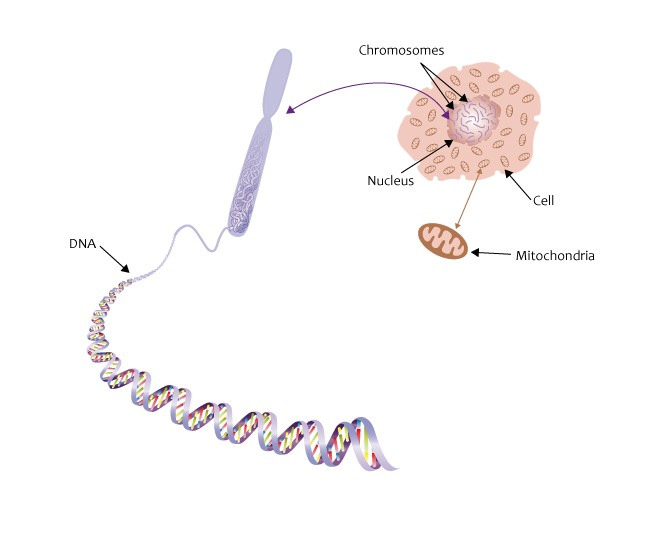
\includegraphics[width=\textwidth,natwidth=627,natheight=614]{dna_condensed.jpg}
   \caption[DNA packaging]{DNA is condensed into chromosomes by forming DNA-protein complexes known chromatin, which is further coiled into thicker fibers called 30nm fibers. The chromosomes reside inside the nucleus of a cell; however, it should be noted that even when chromosomes are not condensed, such as during interphase, there is still the presence of condensed chromatin in the nucleus. Mitochondria contain their own DNA. Image used with permission from Nature Education 2013.}
   \label{fig:dna_condensed}
\end{figure}

\subsection{DNA accessibility}

Chromatin structure and nucleosome positioning are altered in order for the transcriptional and replication machinery to be able to access parts of the genome for transcription. Chromatin structure can be relaxed by biochemically modifying histones, to strengthen or weaken its association with DNA. Generally speaking, there are two major mechanisms by which chromatin is made more accessible via histone modifications:

\begin{enumerate}
   \item Histones can be enzymatically modified by the addition of acetyl, methyl, or phosphate groups.
   \item Histones can be displaced by chromatin remodelling complexes, thereby exposing underlying DNA sequences to polymerases and other enzymes.
\end{enumerate}

Importantly, these two processes are reversible, so modified or remodelled chromatin can be returned to its compact state after transcription and/or replication are complete. The nomenclature for histone modifications is defined by the name of the histone, followed by the single-letter amino acid abbreviation and its position, and then an abbreviation of the enzymatic modification; for example, H3K27ac indicates the acetylation of lysine 27 on H3. Specific histone modifications are associated with different biological states; for example, acetylation removes the positive charge on histones, thereby decreasing the interaction between histones and DNA, loosening chromatin, and leading to transcriptional activation. On the other hand, the tri-methylation of lysine 27 on histone H3, i.e. H3K27me3, is associated with the inhibition of transcription\cite{pmid21652639}. Given that distinct histone modifications can either activate or repress transcription, a ``histone code" has been proposed\cite{pmid11498575} and the profiling of the histone states provides insights into the transcriptional state of a DNA region. Table \ref{table:histone_mod} summarises a list of histone modifications and variants profiled by the ENCODE project\cite{pmid22955616}.

\begin{table}[h]
   \footnotesize
   \begin{tabular}{l l p{5cm}}
Histone modification or variant & Signal characteristics & Putative functions                                                                                                                    \\
H2A.Z                           & Peak                   & Histone protein variant (H2A.Z) associated with regulatory elements with dynamic chromatin                                            \\
H3K4me1                         & Peak/region            & Mark of regulatory elements associated with enhancers and other distal elements, but also enriched downstream of transcription starts \\
H3K4me2                         & Peak                   & Mark of regulatory elements associated with promoters and enhancers                                                                   \\
H3K4me3                         & Peak                   & Mark of regulatory elements primarily associated with promoters/transcription starts                                                  \\
H3K9ac                          & Peak                   & Mark of active regulatory elements with preference for promoters                                                                      \\
H3K9me1                         & Region                 & Preference for the 5′ end of genes                                                                                                    \\
H3K9me3                         & Peak/region            & Repressive mark associated with constitutive heterochromatin and repetitive elements                                                  \\
H3K27ac                         & Peak                   & Mark of active regulatory elements; may distinguish active enhancers and promoters from their inactive counterparts                   \\
H3K27me3                        & Region                 & Repressive mark established by polycomb complex activity associated with repressive domains and silent developmental genes            \\
H3K36me3                        & Region                 & Elongation mark associated with transcribed portions of genes, with preference for 3′ regions after intron 1                          \\
H3K79me2                        & Region                 & Transcription-associated mark, with preference for 5′ end of genes                                                                    \\
H4K20me1                        & Region                 & Preference for 5′ end of genes                                                                                                       
   \end{tabular}
   \caption[Table of histone modifications]{Summary of histone modifications and variants profiled by the ENCODE project\cite{pmid22955616}.}
   \label{table:histone_mod}
\end{table}

\section{DNA sequencing}

DNA sequencing is the process of determining the exact order of nucleotides within a DNA molecule. The first generation of DNA sequencing methods (Sanger and Maxam-Gilbert sequencing) were developed in the 1970s and were very labour intensive, requiring four separate polyacrylamide gel electrophoresis (PAGE) runs, for the determining the sequence of each base. The key feature of Sanger sequencing \cite{pmid271968} was the use of chain-terminating dideoxynucleotide triphosphates (ddNTPs). The structure of a normal nucleotide (dNTP), consists of a 3' hydroxyl (OH) group in the pentose sugar; chain-terminating ddNTPs lack the OH group that is necessary for the formation of the phosphodiester bond between one nucleotide and the next during DNA strand elongation. The idea was to set up a reaction with a mixture of dNTPs [deoxyadenosine triphosphate (dATP), deoxyguanosine triphosphate (dGTP), deoxycytidine triphosphate (dCTP), deoxythymidine triphosphate (dTTP)] and a particular ddNTP in a ratio of 300:1. Most of the times, the DNA will be elongated but if a ddNTP is incorporated into the growing DNA strand, strand elongation is terminated. This results in DNA fragments of varying lengths, where the last base of these fragments corresponding to the ddNTP used. By performing the same reaction for the other three ddNTPs and loading the fragments of each reaction onto separate PAGE lanes, the DNA bases can be deduced by reading the four lanes (Figure ~\ref{fig:sanger_ladder}).

\begin{figure}[!ht]
   \centering
   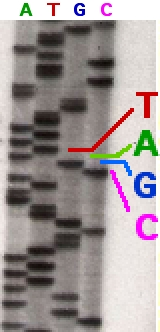
\includegraphics[width=\textwidth,natwidth=160,natheight=332,totalheight=0.20\textheight,keepaspectratio]{sanger_ladder.jpg}
   \caption[Radioactively labelled sequencing gel]{PAGE, which has a 1 bp resolution, is used to separate the radioactively labelled DNA fragments from each reaction using specific chain-terminating ddNTPs. By reading the DNA fragments, the sequence of the DNA can be deduced. Image used under the terms and agreement of the Wikipedia GFDL.}
   \label{fig:sanger_ladder}
\end{figure}

The Maxam-Gilbert sequencing method\cite{pmid265521} relies on the use of chemicals that can cleave specific bases in contrast to chain-terminating ddNTPs. Dimethyl sulfate was used to cleave purine bases (A and G) and hydrazine was used to cleave pyrimidine bases (C and T). To distinguish the purines, an adenine-enhanced cleavage step is carried out, which cleaves adenines preferentially. To distinguish the pyrimidines, NaCl is used with hydrazine to suppress the reaction of thymines. As with Sanger sequencing, the DNA fragments are separated using PAGE, and the DNA bases are deduced by reading the gel.

Sanger sequencing became the \textit{de facto} method for DNA sequencing due to its comparative ease and the use of fewer toxic materials than Maxam-Gilbert sequencing. A further improvement to Sanger sequencing replaced the need to radioactively label the DNA fragments by using chemically synthesised fluorescent oligonucleotide primers\cite{pmid3713851}. Four different fluorophores were used for each ddNTP reaction allowing all four reactions to be co-electrophoresed and the DNA sequence was deduced by reading the fluorescence colours (Figure ~\ref{fig:sanger_sequencing}). The development of a fluorescence detection apparatus linked to a computer that processed the data created the world's first partially automated DNA sequencer\cite{pmid3713851}; this development was key towards the success of the Human Genome Project (HGP). For over 25 years since its inception, Sanger sequencing was the method of choice for DNA sequencing.

\begin{figure}[!ht]
   \centering
   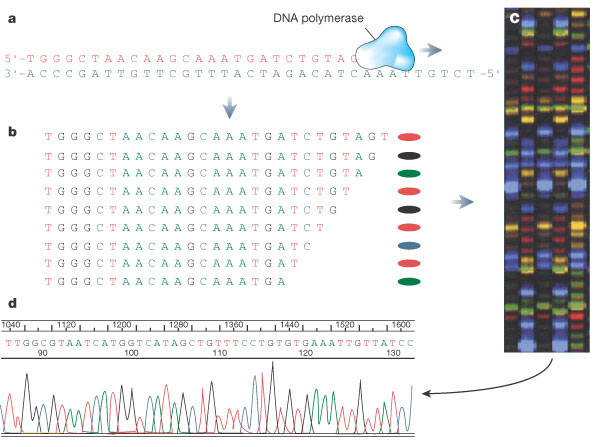
\includegraphics[width=\textwidth,natwidth=600,natheight=447]{sanger_sequencing.jpg}
   \caption[Sanger sequencing]{a) DNA polymerase synthesises a complementary strand of DNA, however when a b) fluorescently labelled chain-terminating ddNTP base is incorporated, synthesis terminates producing DNA fragments of various sizes. c) As each terminator are fluorescently labelled with different dyes, each fragement will fluoresce a particular colour and the d) sequence trace is read by a computer that determines the sequence based on the coloured peaks.}
   \label{fig:sanger_sequencing}
\end{figure}

\subsection{Next-generation sequencing}

The next wave of DNA sequencing techniques, the so-called next-generation (next-gen) or second generation sequencing, started with various strategies that relied on a combination of template preparation, sequencing, and imaging that allowed thousands to billions of sequencing reactions to be performed simultaneo-usly\cite{pmid19997069}. Next-gen sequencing relies on the clonal amplification of templates and uses \textit{in vitro} cloning rather than bacterial cloning; the two most common methods of clonal amplification are emulsion PCR (emPCR)\cite{pmid12857956} and solid-phase amplification\cite{pmid16473845}. With emPCR individual DNA molecules are isolated with primer-coated beads in water-in-oil microreactors and clonal amplification leads to thousands of copies of the DNA molecule in an emulsion. 454 pyrosequencing and Sequencing by Oligonucleotide Ligation and Detection (SOLiD) sequencing employ emPCR and the amplification products are deposited into individual wells for sequencing. Solid-phase amplification relies on a lawn of high-density primers that are covalently attached on a slide surface (also known as a flow cell) and bind to DNA molecules that have been ligated with sequencing adaptors. The two methods allow each DNA template to be spatially separated and allow massively parallel sequencing to take place.

Sequencing can take place via the use of DNA polymerase, which is commonly known as sequencing-by-synthesis (SBS), or via the use of DNA ligase, which is known as sequencing-by-ligation (SBL). SBS can be further classified into cyclic reversible termination (CRT), single-nucleotide addition (SNA), and real-time sequencing\cite{pmid19997069}. CRT uses reversible terminators and initial developments used the dideoxynucleotides chain terminators used in Sanger sequencing. The concept of CRT is that a DNA polymerase incorporates one fluorescently modified nucleotide, which has a reversible terminator that terminates DNA synthesis. Unincorporated nucleotides are washed away and fluorescence imaging takes place to determine the identity of the incorporated nucleotide. The last step removes or cleaves the reversible terminator and the fluorescent dye, and the cycle is repeated. The CRT method is used in Solexa/Illumina and Helicos single-molecule fluorescent sequencing. SBL relies on DNA ligase and uses either one-base-encoded or two-base-encoded probes that are fluorescently labelled. The probes hybridise to its complementary sequence on the primed template and DNA ligase is added to join the probe to the primer. Non-ligated probes are washed away followed by fluorescence imaging and cleavage of the fluorescent dye and the cycle is repeated. The SBL method is used in SOLiD sequencing.

\subsection{Third generation sequencing and beyond}

The third generation of sequencing refers to single-molecule sequencing technologies, which has the capacity for generating longer read lengths at potentially cheaper costs\cite{pmid20858600}. One of the major advantages of single-molecule sequencing is that PCR is not required, and therefore amplification biases and PCR mutations are eliminated. Furthermore, by employing third generation sequencing, quantitative applications of sequencing, such as RNA sequencing, can give a much more representative picture of the true abundance of RNA molecules. The HeliScope sequencer was the first commercially available single-molecule sequencer, which was based on the work of Stephen Quake and colleagues\cite{pmid12651960}. HeliScope sequencing utilises billions of primed single-molecule templates that are covalently attached to a solid support and uses CRT but with slight differences from Solexa/Illumina sequencing. HeliScope sequencing uses Helicos Virtual Terminators, which differ from the reversible terminators used in Solexa/Illumina sequencing and dye labelled nucleotides are added individually in the predetermined order of C, T, A, and G, followed by fluorescence imaging.

With the advent of high-throughput sequencing we now have the capacity to sequence an entire human genome in a matter of days. In addition, we have just recently arrived in the \$1,000 genome era, whereby we can sequence the entire genome of an individual at a 30x depth (the minimum depth required for clinical applications) for around \$1,000 US dollars (USD). In contrast, the Human Genome Project (HGP), which gave us the first glimpse of the human genome\cite{lander2001initial} costed approximately 2.7 billion fiscal year 1991 US dollars\cite{nhgri2010cost}. Further developments in sequencing by various companies are aiming towards longer read lengths at a higher output (Figure ~\ref{fig:dev_next_gen}). Currently, different sequencers either have very long reads but at a low-throughput or have a high-throughput of shorter reads; as such, each sequencer fills a particular niche. \textit{De novo} assembly of genomes requires longer reads for less ambiguity and the quantification of RNA requires higher throughput in order to accurately sample the vast RNA population.

\begin{figure}[!ht]
   \centering
   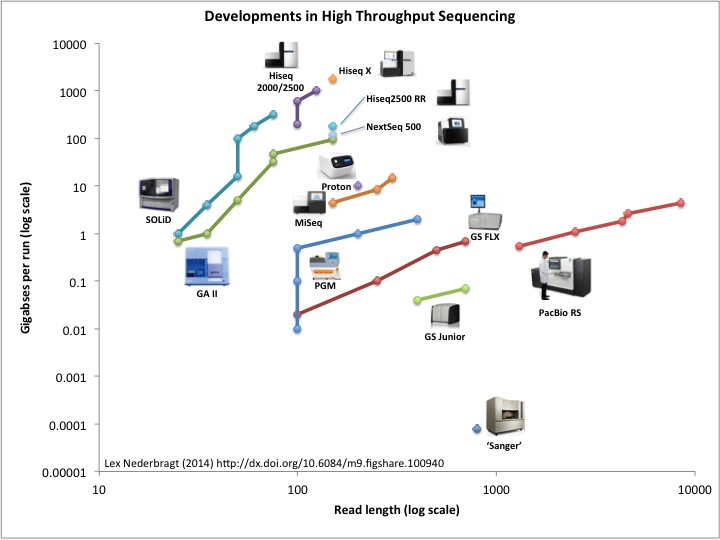
\includegraphics[width=\textwidth,natwidth=720,natheight=540]{developments-in-next-generation-sequencing.jpg}
   \caption[Developments in next generation sequencing]{Log read length versus log gigabases per run for various high-throughput sequencer\cite{Nederbragt2012}. Currently, the HiSeq X, the sequencer that bought us into the \$1,000 genome era, provides the highest throughput.}
   \label{fig:dev_next_gen}
\end{figure}

\section{Analysis of transcript expression}

One of the first methods for detecting a specific transcript within a sample was Northern blotting\cite{pmid414220}. This technique involves electrophoretic separation of purified RNA, followed by immobilisation onto a blotting membrane, and detection by hybridisation of a specific probe that is complementary to part of the target sequence. Northern blotting enables the detection of a specific RNA and by comparing the strength of signals from different samples, the relative amount of a specific transcript can be estimated. This estimate assumes that an equivalent amount of total RNA was used per sample and is usually verified by using a probe that detects a housekeeping transcript that is constitutively expressed. Northern blotting still remains as a lasting method for determining the size of a specific transcript and used for detecting alternatively spliced transcripts. It should be noted that the amount of a specific transcript in a cell at a given time is not only influenced by the rate of transcription but also by the stability of the transcript; a rapidly degraded transcript may appear to be lowly transcribed. In addition, protein-coding transcript levels do not necessarily correlate with the level of protein that is encoded by the transcript.

However, Northern blotting is not very sensitive for estimating transcript abundance. The most sensitive method of detecting specific transcript levels is quantitative real-time polymerase chain reaction (qRT-PCR), which is able to detect transcripts in a single cell. The method is based on measuring the number of cycles that is required for the formation of a detectable amount of product, which is known as the cycle threshold ($C_{t}$) value; higher amounts of initial template will result in lower $C_{t}$ values. As with Northern blotting, a parallel qRT-PCR is performed on a housekeeping transcript to assess the amount of total RNA before comparing assays from different samples. It should be ensured that the polymerase chain reaction (PCR) step is equally efficient for different transcripts, as a more efficient PCR will result in a lower $C_{t}$ value compared to a less efficient PCR.

\subsection{Transcriptome profiling}

The transcriptome is the complete collection of transcripts in a cell at a specific time point; transcriptome profiling refers to the expression profiling of all transcripts. One of the first technologies that allowed the simultaneous profiling of thousands of transcripts was microarrays\cite{pmid7569999}, which is a hybridization-based approach. DNA probes that are complementary to specific DNA sequences, such as RNA transcripts or genomic regions, are attached to a solid surface and fluorescently labelled target sequences are hybridised onto the surface. Target sequences complementary to the probe sequences will hybridise to the probe and the signal intensity provides a measure of the expression strength of a particular transcript. In one of the first studies that employed microarrays, researchers were able to observe the change in expression patterns of 700 mRNAs during a switch from aerobic to anaerobic respiration in yeast cells\cite{pmid9381177}. However, microarrays have several limitations, which includes requiring \textit{a priori} knowledge of the genome or transcript sequences for the design of probes, high background levels from cross-hybridisation\cite{pmid16749918}, and a limited dynamic range in quantifying expression.

In contrast to the hybridisation approach of microarrays for transcriptome profiling are the sequence-based technologies, which can be grouped into whole transcriptome shotgun sequencing or tag-based sequencing. A technology called Serial Analysis of Gene Expression (SAGE)\cite{pmid7570003} was the first tag-based approach that could be used for transcriptome profiling. SAGE involved obtaining short fragments derived from complementary DNA (cDNA), followed by concatenation and cloning, and sequencing. The concatenation step allowed 10-20 SAGE tags, which were 9 to 10 bp long and generally corresponded to the 3' end of the transcripts, to be cloned into each plasmid and reduced the cost of sequencing by one order of magnitude. A similar technology known as Massive Parallel Signature Sequencing (MPSS), was later developed, which is in essence similar to SAGE but uses different biochemical manipulations and sequencing approach\cite{pmid10835600}. MPSS was an improvement to SAGE in that it produced longer tags (16-20 bp) and libraries that were 20 times larger than typical SAGE libraries\cite{pmid10835600}. The SAGE approach also gave rise to Cap Analysis Gene Expression (CAGE)\cite{pmid14663149}, which combines the tagging strategies of SAGE with a molecular technique known as Cap-Trapper\cite{pmid8938445,pmid9179497}, which allows the capturing of all RNAs that have a cap structure. The CAGE protocol captures all capped transcripts and sequences a short tag that corresponds to the 5' end of an RNA transcript (Figure ~\ref{fig:cage_protocol}). Whole transcriptome shotgun sequencing or simply RNA sequencing (RNA-Seq), refers to the fragmentation of RNA followed by deep-sequencing on next-gen sequencing platforms\cite{pmid19015660}. Typically, RNA-Seq approaches focus on transcripts with a poly-A tail; the poly-A enrichment step avoids rRNA sequences, which make up a large fraction of the total RNA population.

\begin{figure}[!ht]
   \centering
   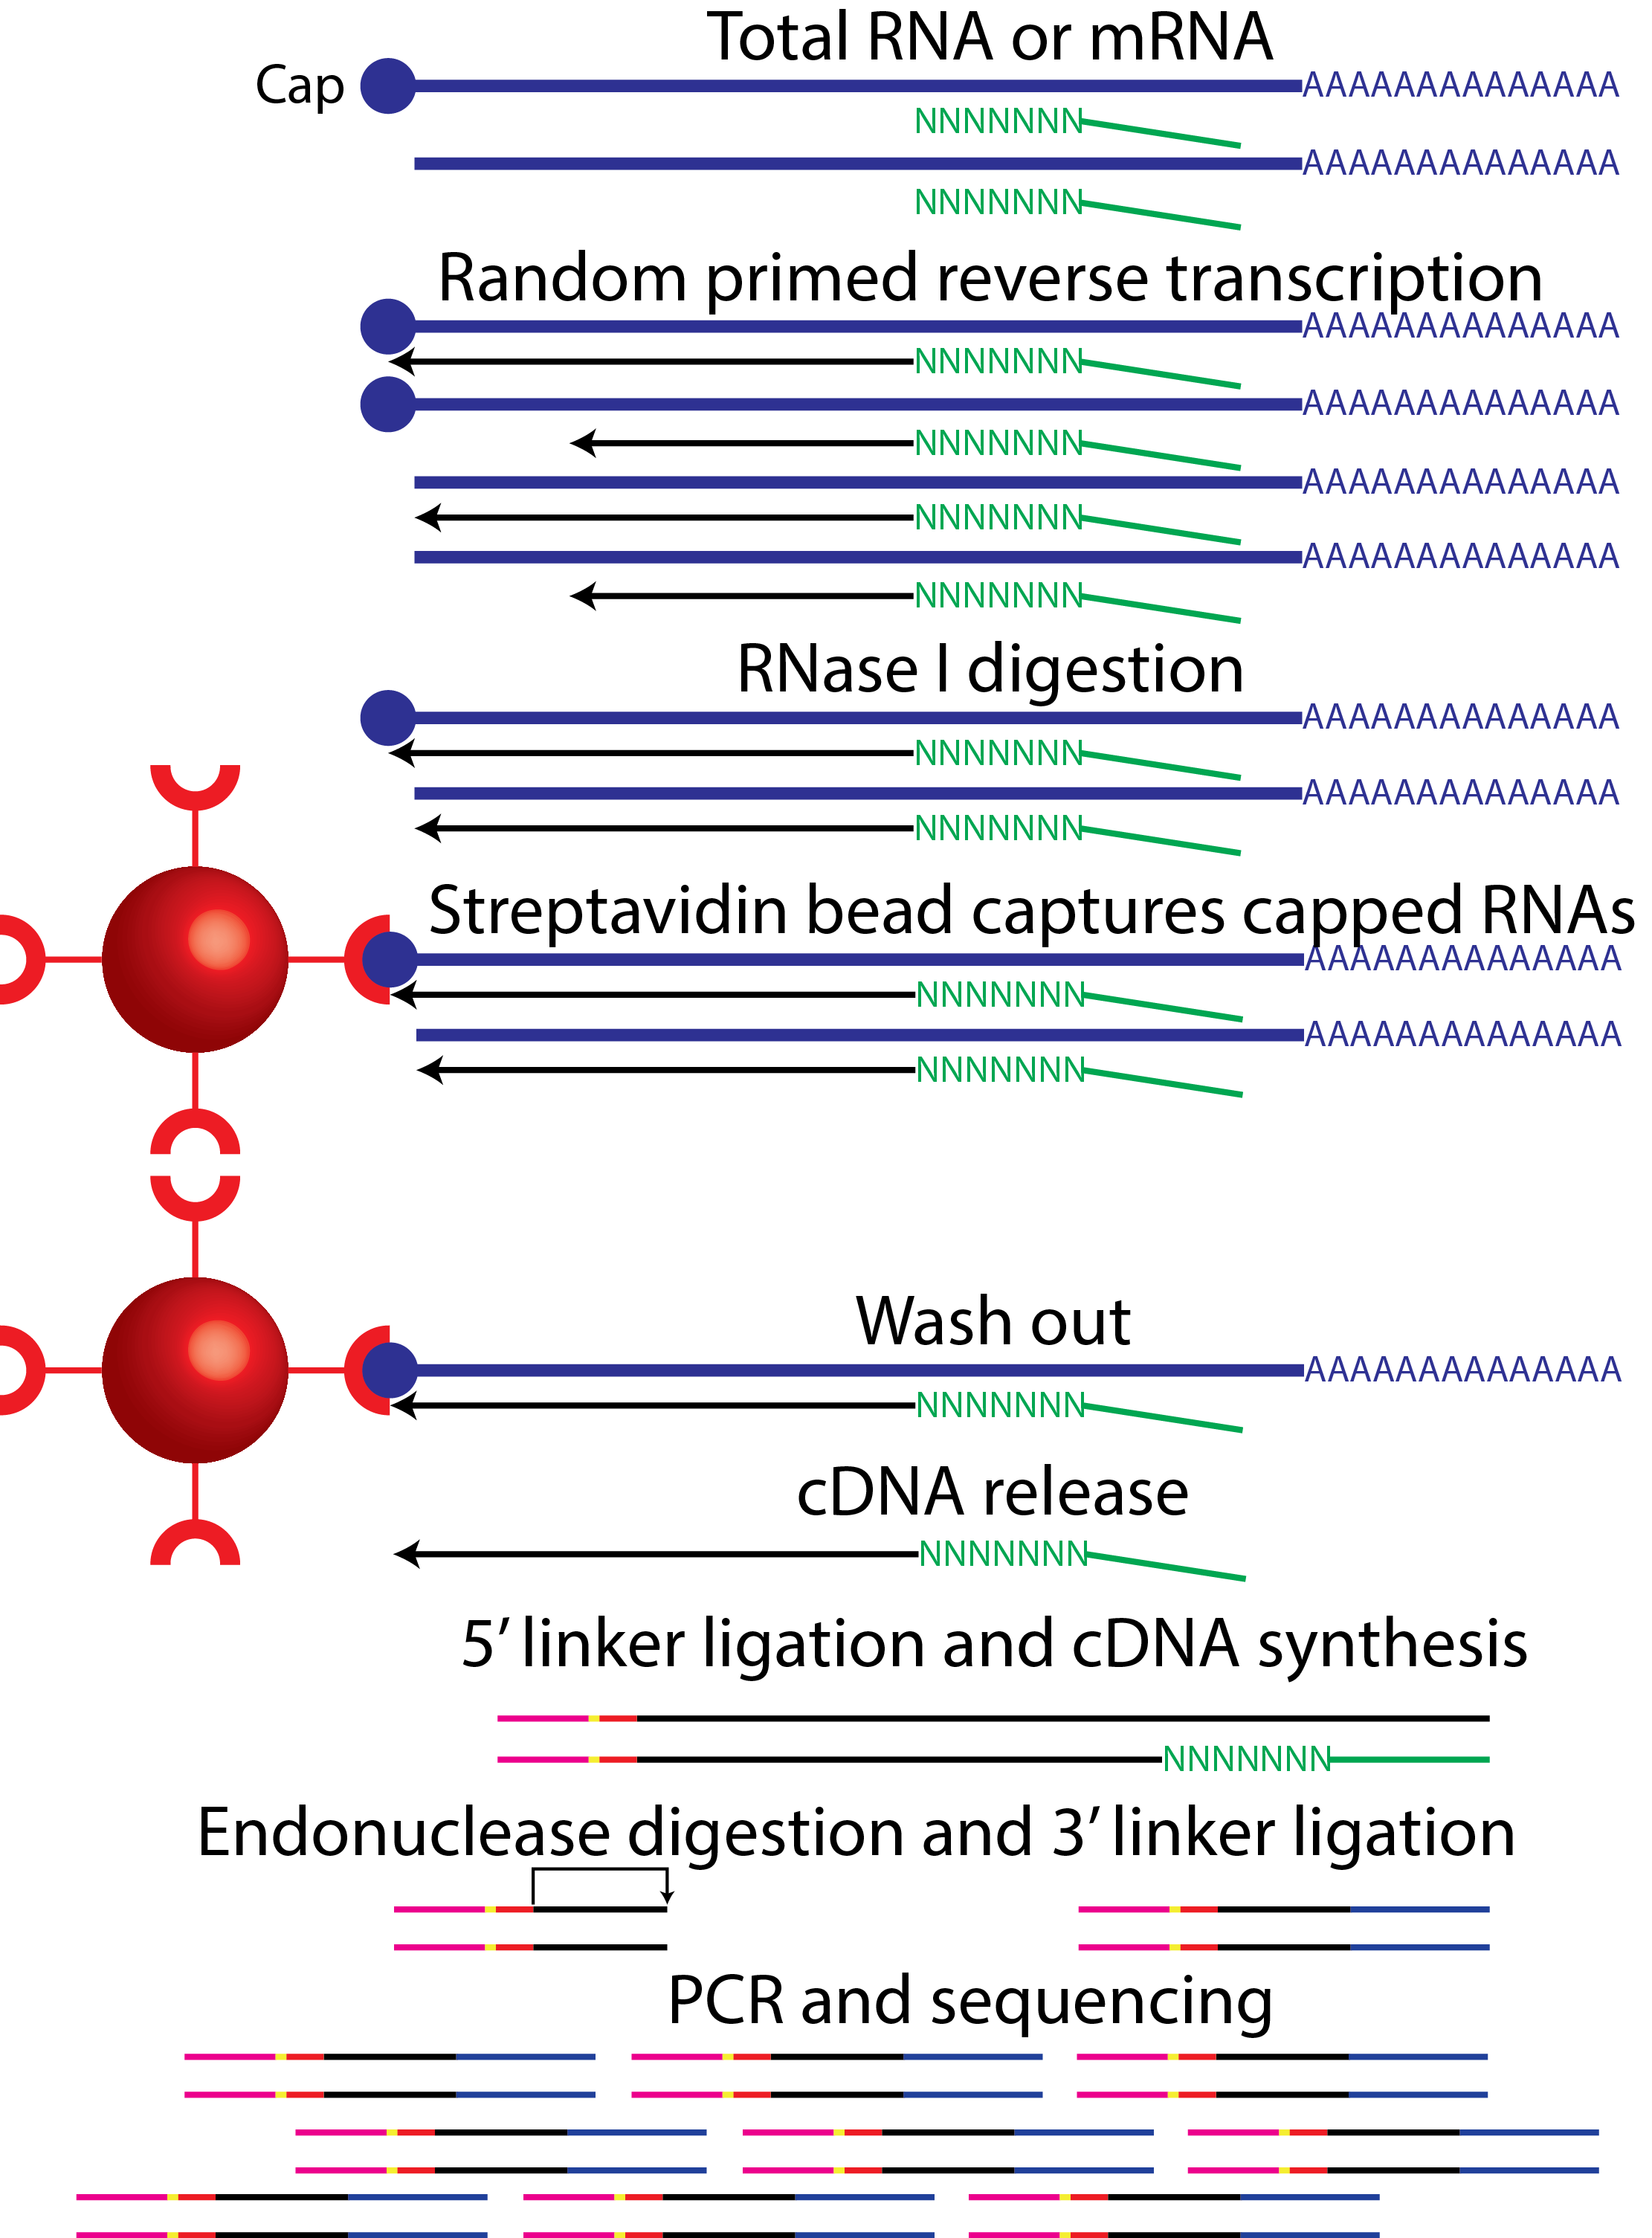
\includegraphics[width=\textwidth,natwidth=2254,natheight=3051,totalheight=0.65\textheight,keepaspectratio]{cage_protocol.png}
   \caption[Cap Analysis Gene Expression protocol]{The Cap Analysis Gene Expression (CAGE) protocol starts with synthesising cDNA from either total RNA or mRNA by using random or oligo dT primers (only random primers are shown here). Reverse transcription takes place in RNAs with or without a cap and to full or partial completion; the RNase I digestion removes partially reverse transcribed RNA as they are not protected by a full double strand. The 5' end of cDNAs are selected by streptavidin beads and unbound cDNA are washed out. After release from the bead, a linker is attached to the 5' end of the single-stranded cDNA; this linker contains recognition sites that allow the endonuclease cleavage. Lastly a linker is attached to the 3' end of the tag sequence, which is amplified and directly sequenced.}
   \label{fig:cage_protocol}
\end{figure}

\subsection{Blah}

The classical view of transcription initiation was that transcription began at a single position at TA-rich regions known as the TATA-box. One of the major findings made using the CAGE technology was that not all transcription initiation events occurred at a single position\cite{pmid16645617}. While the classical TATA-box promoters mostly initiated from a single position (which were termed sharp promoters), promoters that were CG-rich (in particular CpG islands) showed initiation events across a stretch of sequence (these were termed broad promoters). Initially these CAGE tags were thought to be noise, however, these TSSs were highly consistent in orthologous mouse and human promoters, and sharp and broad promoters were consistently detected in various libraries\cite{pmid16645617}. In addition, this initial survey of the transcriptional landscape in mammalian genomes identified many novel mRNAs and non-coding RNAs that had not been previously characterised\cite{pmid16141072}. CAGE has also been applied to study the dynamics of TSS usage throughout a time course of growth arrest and differentiation\cite{pmid19377474}.

The latest FANTOM project, FANTOM5, used CAGE with a single-molecule sequencer, to profile a large panel of mammalian primary cells, tissues, and cell lines\cite{pmid24670764}. CAGE was also used as part of the ENCODE project to study subcellular localisation of RNAs\cite{pmid22955620}.

Using deep sequencing (deepCAGE), the FANTOM4 study measured the genome-wide dynamics of transcription-start-site usage in the human monocytic cell line THP-1 throughout a time course of growth arrest and differentiation. Modeling the expression dynamics in terms of predicted cis-regulatory sites, we identified the key transcription regulators, their time-dependent activities and target genes. Systematic siRNA knockdown of 52 transcription factors confirmed the roles of individual factors in the regulatory network. Our results indicate that cellular states are constrained by complex networks involving both positive and negative regulatory interactions among substantial numbers of transcription factors and that no single transcription factor is both necessary and sufficient to drive the differentiation process.

Two variants of CAGE include nanoCAGE\cite{pmid20543846} and HeliScopeCAGE\cite{pmid21596820}; the latter variant was specifically developed and used for the FANTOM5 project. Briefly, nanoCAGE utilises the template-switching method\cite{pmid11314272} instead of Cap-Trapper for capturing the TSS of RNAs. Template-switching allows a simplification of the CAGE protocol and requires a much smaller amount of starting RNA, to the level of RNA content present in single cells (10 picogram/cell). HeliScopeCAGE utilises Cap-Trapper but without the enzymatic tag cleavage and PCR amplification, and the capped 5' ends of the cDNA are directly sequenced on the HeliScope sequencer. The automation of HeliScopeCAGE\cite{pmid22303458} allowed the large panel of samples to be sequenced for the FANTOM5 project.

\subsection{Transcriptional products}

The idea of a gene dates back to Gregor Mendel when he demonstrated in his plant breeding experiments that discrete traits could be inherited from parents to offspring. While the mechanism of inheritance was not clear at that time, these heritable traits became known as a gene.

The definition of a gene has evolved with our increasing knowledge of genetics and biochemistry\cite{pmid17567988}.

In 1941, George Beadle and Edward Tatum observed that mutations in Neurospora genes would cause defects in different steps of metabolic pathways\cite{Beadle15111941}. The demonstration of how genes directed the synthesis of enzymes later became known as the ``one gene, one polypeptide" hypothesis, where each gene was responsible for producing a single protein in a biochemical pathway.

\subsection{Pervasive transcription}

1% ENCODE \cite{pmid17571346}.

\begin{itemize}
   \item Pervasive transcription refers to the observation that a large fraction of mammalian genomes are transcribed
   \item Is this a consequence of RNA Pol II randomly colliding with open chromatin or transcription factors binding to random sequences of DNA that resemble the TFBS? Is this simply noise?
   \item How do we ascribe function to these pervasively transcribed elements or argue against noise?
\end{itemize}

Common criteria for ascribing function

\begin{itemize}
   \item Context-specific transcription
   \item A random transcript would not become active under a specific condition
   \item Tissue specificity
   \item Developmental stage specificity
   \item Stimulus-specific activation, such as in response to stress
   \item Positional information
   \item Proximity of DNA sequences to significant sites, such as to known protein-coding transcripts, implies a regulatory role
   \item Sequence conservation
   \item Instances of conservation are evidence of purifying selection
   \item Experimental manipulation
   \item Observable phenotypic change with experimental manipulation
   \item The observation of context-specific expression patterns as a criteria for function can be countered by the fact that:
   \item Different transcription factors are present in different cell types and at different stages of development.
   \item The accessibility of different parts of the genome vary from cell type to cell type and at different kinds of development.
   \item Molecular assays
   \item Transcript expression can be assayed using qRT-PCR
   \item Reporter-gene assays, such as placing putative regulatory sequences upstream of a reporter gene
   \item Tissue or intracellular localisation of transcripts can be determined using RNA FISH
   \item Biological assays
   \item assay how a genetic element produces a measurable phenotypic effect by the
   \item Use of cell lines to knockdown or transfect cells with a specific transcript
   \item Use of animal models to knock-out or knock-in transcripts
\end{itemize}

\subsection{Non-coding RNAs}

The FANTOM project began as an initiative to sequence and annotate mouse full-length complementary DNA (cDNA)\cite{pmid11217851}. At the end of the first FANTOM project, a collection of approximately 21,000 full-length cDNAs were annotated and made available. By the time of FANTOM2, a continuation of the FANTOM project, the number of mouse full-length cDNAs had increased to approximately 61,000 and revealed a transcriptome that was dominated by transcripts that had no apparent coding potential and thus were labelled as transcripts of unknown function (TUFs)\cite{pmid12466851}. FANTOM3 provided the last update to the mouse full-length cDNAs, increasing the number to roughly 100,000 cDNAs\cite{pmid16141072}. Using the Coding-Potential Assessment Tool (CPAT)\cite{pmid23335781}, which is a tool that assesses the coding potential of an input sequence, 38.6\% of the FANTOM3 mouse full-length cDNAs were deemed to have a very low coding potential (coding probability of less than 0.2) (Figure ~\ref{fig:fantom3_coding_prob}). This corroborates previous analyses of the mouse full-length cDNAs performed during the FANTOM2 project.

\begin{figure}[!ht]
   \centering
   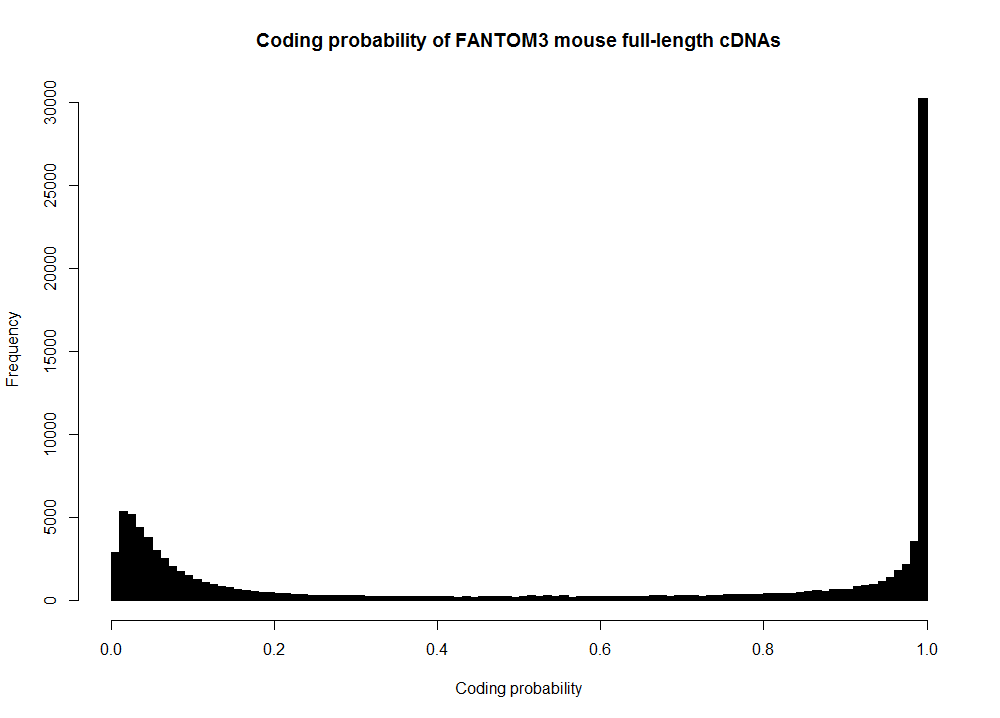
\includegraphics[width=\textwidth,natwidth=1000,natheight=718]{fantom3_coding_probability.png}
   \caption[Coding probability of FANTOM3 mouse cDNAs]{CPAT is a tool that assesses the probability that an input sequence is coding or non-coding by examining the open reading frame (ORF) length and coverage, the Fickett statistic\cite{pmid7145702}, and the hexamer usage. Shown above is the distribution of CPAT coding probabilities for the entire set of FANTOM3 mouse full-length cDNAs\cite{tang2014fantom3codingprob}.}
   \label{fig:fantom3_coding_prob}
\end{figure}

High-throughput methods of transcriptome analysis such as RNA-Seq have also revealed a large number of previously non-annotated transcripts with very low coding potential. While there is no official nomenclature on the naming of such transcripts, they have been known as non-coding RNA and broadly broken down into two classes: short and long non-coding RNA. Long non-coding RNA (lncRNA) are defined as non-protein-coding RNAs that are \textgreater200 nucleotides in length; this size corresponds to the commonly used cutoff for size selection in biochemical fractionations. Short non-coding RNA are defined as non-protein-coding RNAs that are \textless200 nucleotides. NcRNAs exist as single-strand nucleic acid molecules, which tend to fold on itself due to the hydrophobic nature of bases, to form localised double-stranded regions that form structures called hairpins or stem-loop structures. The classical non-coding RNA found in both prokaryotes and eukaryotes are the ribosomal RNAs and transfer RNAs, both of which are both involved in protein synthesis. Many of the recently characterised ncRNAs have regulatory roles instead\cite{pmid24776770}.

The most well studied class of short ncRNAs are the micro-RNAs (miRNAs), which were first observed in Caenorhabditis elegans\cite{pmid8252621}. MiRNAs are typically 20-24 nucleotides in length and functions as regulators of expression by base-pairing with complementary sequences within mRNAs (commonly to the 3' untranslated region (UTR)). The biogenesis of miRNAs begins transcription of the miRNA gene by Pol II or Pol III, which forms the primary miRNA (pri-miRNA). The pri-miRNA is cleaved by an enzyme called Drosha\cite{pmid14508493} to produce a characteristic stem-loop structure of about 70 bps, known as the precursor miRNA (pre-miRNA). The pre-miRNA is then exported into the cytoplasm and is further cleavage by an enzyme called Dicer\cite{pmid11201747}, producing the mature miRNA. Another class of well known short ncRNAs are the Piwi-interacting RNA (piRNA), which were first observed in drosophila\cite{pmid11470406}. PiRNA are typically between 24 and 32 nucleotides long and are thought to be involved in gene silencing, especially in silencing transposable elements (TEs), by forming the piRNA-induced silencing complex (piRISC). The sequence of many piRNAs are antisense to transposon sequences because they are actually derived from TEs. In fact when they were first discovered in drosophila, they were termed repeat-associated small interfering RNAs (rasiRNA). One theory of piRNA biogenesis states that piRNAs are processed from single-stranded RNA precursors coming from particular intergenic repetitive elements, such as TEs\cite{pmid21427766}.

\section{Repetitive mammalian genomes}

The discovery that cells contained a large fraction of repetitive DNA was made by measuring the reassociation rates of DNA strands after denaturation\cite{Britten1968}. Through the mouse\cite{pmid12466850} and human\cite{venter2001sequence, lander2001initial} genome sequencing projects, it was confirmed that a large majority of the mouse and human genome are made up of repetitive elements (REs). There are two major groups of repeats: tandem repeats, which include different classes of satellite repeats, and interspersed repeats, which are mostly made up of transposable elements (TEs)\cite{pmid9666329}. Methods for the identification of TEs include \textit{de novo}, homology, structure, and comparative genomic based methods\cite{Bergman01112007}. A popular homology-based software for the annotation of TEs is RepeatMasker, which identifies REs by searching against a database\cite{pmid19274634}. The Repbase Update database\cite{pmid16093699} contains consensus sequences of REs from diverse eukayotic genomes and is commonly used by RepeatMasker as the input database. A comparison of REs detected by RepeatMasker amongst 66 vertebrate genomes, shows that the coverage of REs in the human genome is relatively high (Figure ~\ref{fig:repeat_coverage_vertebrate_genome}). However, the detection ability of RepeatMasker is dependent on the database containing the REs and the alignment tool.

\begin{figure}[!ht]
   \centering
   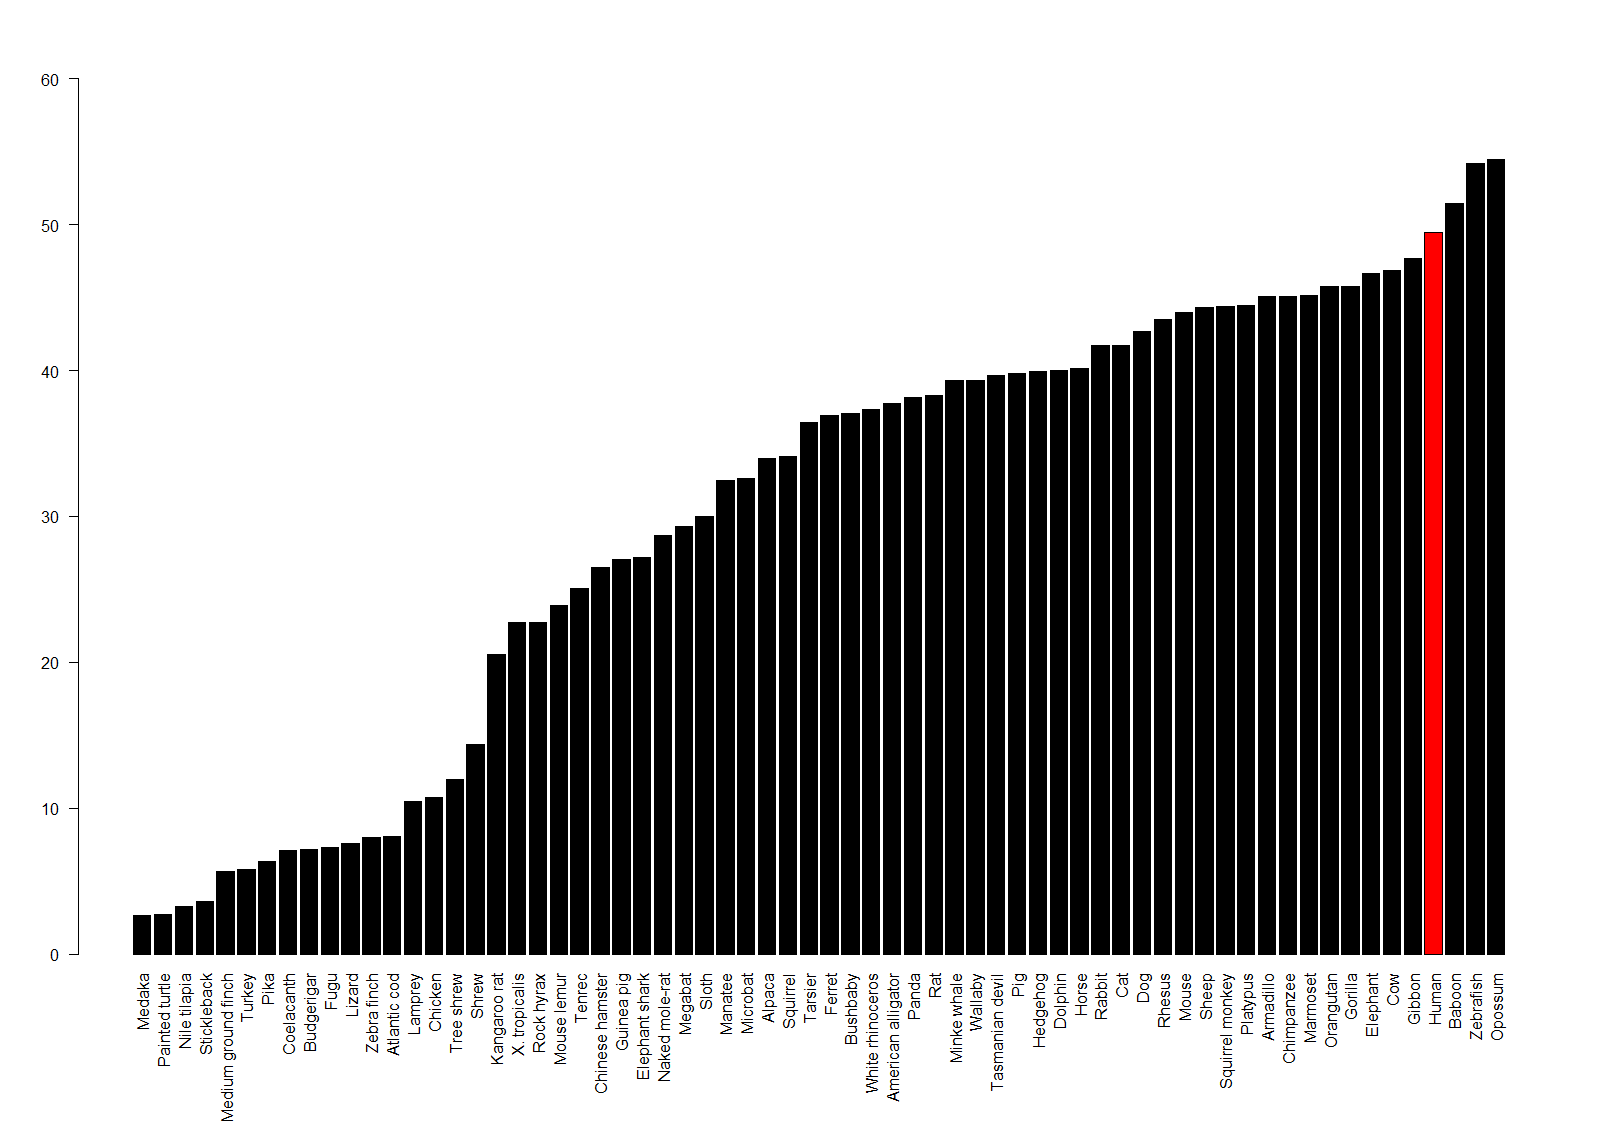
\includegraphics[width=\textwidth,natwidth=1600,natheight=1148]{repeat_coverage_vertebrate_genome.png}
   \caption[Coverage of repetitive elements in vertebrate genomes]{The total coverage of repetitive element in 66 vertebrate genomes as annotated by RepeatMasker in the respective genomes, where the human fraction is shown in red\cite{tang2014repcoverage}.}
   \label{fig:repeat_coverage_vertebrate_genome}
\end{figure}

There are two classes of transposons: Class I TEs or retrotransposons, which are first transcribed into RNA and then reverse transcribed back to DNA (a copy-and-paste mechanism), and Class II TEs or DNA transposons, which simply cut-and-paste their DNA sequence from one location to another via transposase enzymes. Given that retrotransposons are able to produce a copy of itself before propagation, they are more numerous than DNA transposons and may comprise over two-thirds of the human genome\cite{pmid22144907}. Historically, TEs have been labelled as purely selfish elements that have no function or provide no selective advantage to an organism\cite{doolittle1980selfish, orgel1980selfish}. However it should be pointed out that the authors did leave open the possibility that some TEs may become useful:

\epigraph{``It would be surprising if the host genome did not occasionally find some use for particular selfish DNA sequences, especially if there were many different sequences widely distributed over the chromosomes. One obvious use $\ldots$ would be for control purposes at one level or another. This seems more than plausible."}{--- \textup{Orgel and Crick 1980}}

Indeed there is an increasing appreciation of TEs serving as a source for evolutionary innovation\cite{Muotri15102007, pmid18368054}. TEs may become exapted, a process where TE have acquired function, which may be positively selected for. For example, TEs may acquire a regulatory function by providing TFBSs for TFs and thereby drive the expression of a nearby DNA. In a study examining the binding sites of various TFs, it was discovered that REs can provide binding sites for TFs; these sites were termed repeat-associated binding sites (RABS)\cite{pmid18682548}. Importantly, the study demonstrated that RABS are over-represented in proximity of regulated genes and that the binding motifs within these repeats have undergone evolutionary selection. CAGE also demonstrated that many TEs are indeed transcribed in a tissue-specific manner and served as alternative promoters\cite{pmid19377475}. Corroborating with tissue-specific expression of TEs was a study demonstrating that methylation patterns of TEs differed amongst different tissues\cite{pmid23708189}. Though not a definitive measure, tissue-specific expression patterns are still useful for separating signal from noise as expression patterns are not a consequence of random experimental noise.

\subsection{Junk DNA}

The origin of the term ``junk DNA" is usually attributed to Susumu Ohno\cite{pmid5065367}, who used it to describe pseudogenes, which are gene copies that have no known biological function. In its modern day usage, ``junk DNA" is used to describe DNA sequence that does not play a functional role in an organism. Junk DNA has recently been bought into the spotlight by the ENCODE project, which reported that 80\% of the human genome has a biochemical function\cite{pmid22955616} and was translated as an eulogy for junk DNA\cite{Pennisi07092012}. ENCODE's reported findings were criticised since having biochemical activity alone is insufficient for claiming function\cite{pmid23431001, pmid23479647, Eddy2012}. Furthermore, in terms of mutational load it is impossible that 80\% of the human genome is functional as this would lead to mutational meltdown\cite{pmid24809441}. The idea, which was pointed out by Susumu Ohno\cite{pmid5065367}, was that given a fixed mutation rate (each locus has a $10^{-5}$ probability of sustaining a deleterious mutation), the number of functional loci in the human genome must reach a limit due to genetic load. He predicted that mammalian genomes could not have more than 30,000 loci under selection as this would guarantee a progressive decline in genetic fitness, leading to extinction. However, the contrary, that 80\% of the ``functional" sites reported by ENCODE are non-functional is probably not true. Based on sequence conservation, it seems that around 5-20\% of the human genome is under detectable selective pressure\cite{Eddy2012}. As for the question of why there is so much junk DNA in the human genome, Sydney Brenner gives us his take on the subject in his Nobel lecture\cite{brennernobellecture}:

\epigraph{``I had also come to the conclusion that most of the human genome was junk, a form of rubbish which, unlike garbage, is not thrown away."}{--- \textup{Sydney Brenner 2002}}

\section{Bioinformatics and genomics}

Modern day high-throughput sequencers generate a large amount of data; for example, in the blood transcriptome project (Chapter 7), one lane of sequencing on the HiSeq2000 produced 74.5 million CAGE reads (using 15 gigabytes of storage space when uncompressed). To deal with data at this scale, dedicated informatics tools for storing, managing, and the analysis of such data sets are absolutely necessary. Bioinformatics can be thought of as a subset of informatics that deals with biological data, though historically it was defined as ``the study of informatic processes in biotic systems"\cite{pmid21483479}. The HGP was one of the first large scale international research efforts, which demonstrated how bioinformatics was crucial towards the successful completion of the project\cite{stein1996perl}. The HGP also set the stage for data sharing, whereby important principles were established by an international assortment of genome-research leaders towards the rapid and public sharing of human genome information, which are collectively known as the ``Bermuda Principles". These set of commitments left a lasting legacy in large genomic science projects such as The International HapMap Project, ENCODE and modENCODE, and The Cancer Genome Atlas where data was made freely available prior to publication\cite{contreras2011bermuda}. By opening such resources, researchers are able to integrate these datasets with their own research.

\subsection{Standard tools and formats}

The development of standards is another crucial aspect in bioinformatics, for consistency and interoperability. Several standards have been established in the genomics field. The FASTQ format was formally defined in 2010\cite{pmid20015970} and has become the \textit{de facto} format for storing raw high-throughput sequencing output. FASTQ is similar to the FASTA format but with the addition of quality scores, known as the Phred quality score, for each nucleotides. The Sequence Alignment/Map (SAM) format\cite{pmid19505943} is the standard file format for storing sequence alignments. This format has information on how a sequencing read aligns to a reference sequence, such as the mapping location and quality. The open source program SAMTools\cite{Li15082009}, provides various utilities for processing alignments in the SAM format. The BED format\cite{bedformat} is also another commonly used standard for storing the location of a set of features within a reference and has been made popular by the UCSC Genome Browser\cite{Kent01062002}. Due to the popularity of the BED format, a suite of tools released as BEDTools\cite{pmid20110278}, provides various routines for comparing genomic features stored in BED format. There are various tools for the alignment of high-throughput sequencing reads. Traditional tools such as BLAST\cite{pmid2231712} and BLAT\cite{pmid11932250} are unable to cope with the large quantity and short length of reads from high-throughput sequencers. One popular short-read alignment tool, BWA\cite{pmid19451168}, implements the Burrows–Wheeler transform to deal with millions to billions of short reads. The Burrows-Wheeler transform allows a large mammalian genome, for example human, to be indexed and stored efficiently into memory\cite{pmid19430453}.

\subsection{Analysing expression datasets}

Typically, expression data sets are stored as matrices; for example, if we let $A$ be an $m \times n$ matrix, where $a_{ij}$ are elements of $A$, then the $i^{th}$ row would represent the transcriptional response of the $i^{th}$ transcript and the $j^{th}$ column would represent the expression profile of the $j^{th}$ assay:

\begin{align*}
   A = \begin{bmatrix} a_{11} & \cdots & a_{1j} & \cdots & a_{1n} \\
   . && . && . \\
   a_{i1} & \cdots & a_{ij} & \cdots & a_{in} \\
   . && . && . \\
   a_{m1} & \cdots & a_{mj} & \cdots & a_{mn} \end{bmatrix}
\end{align*}

For the comparison of different CAGE assays, it is necessary to normalise the data. The simplest method of normalisation is by counts or tags per million (TPM). To normalise by TPM the $i^{th}$ gene in the $j^{th}$ assay:

\begin{align*}
   TPM_{a_{ij}} = \frac{a_{ij} \times 1000000}{\sum_{i=1}^{m}{a_{mj}}}
\end{align*}

Several types of analyses can be conducted on this expression matrix. When the assays can be grouped, for example, into a set of controls versus a set of treatments, a differential expression analysis can be conducted between the two groups. In order to call differential expression for a given transcript, it is important to assess whether the variation observed between the two groups is significantly larger than the variation observed in the assays from the same group. RNA-Seq expression data is digital, meaning that expression levels are discrete, and the variance can be modelled using discrete probability distributions. In a pioneering study examining the reproducibility of RNA-Seq, it was noted that the variation between technical replicates was close to the shot noise limit\cite{pmid18550803}. Thus it was suggested that the Poisson model was sufficient in modelling the variance and used for testing differential expression. However, it was demonstrated that the Poisson model underestimated the effects of biological variability, i.e. the variation between two different biological samples is greater than Poisson variation\cite{20979621}. This can be accounted for by modelling variance under a negative binomial model, which has been implemented for differential expression analysis in the edgeR package\cite{pmid19910308} from Bioconductor\cite{pmid15461798}.

By far the most popular visual representation of expression data is through heatmaps, which transforms the expression matrix into colours representing the relative expression strength. Heatmaps are commonly displayed with dendrograms that represent the hierarchical clustering of different transcripts and assays\cite{pmid9843981}. This sort of visualisation is intuitive and transcripts with a similar transcriptional response can be immediately identified. Hierarchical clustering relies on a distance matrix, which contains measurements of how similar or dissimilar each transcript or assay is from every other transcript or assay. There are several different distance measures, including Euclidean, maximum, Manhattan, Canberra, and Minkowski. Correlation measures such as Pearson's product-moment correlation coefficient and Spearman's rank correlation coefficient can also be used as distance measures. Correlations can be used to imply co-expression, i.e. transcripts with a similar transcriptional response are assumed to be co-expressed, and co-expression matrices can be visualised as graphs, where each node is a transcript and an edge connects transcripts that have a correlation above a certain threshold.
